\documentclass[../../labo_tp5_main.tex]{subfiles}

\begin{document}

%capítulo
\section{Ejercicio 6}

En Argentina, el espectro de FM (de 88MHz a 108MHz)se divide en 7 categor\'ias (de la A a la G) seg\'un su radio de servicio, es decir hasta d\'onde la potencia de la estaci\'on se mantiene dentro de los 48$\frac{dB\mu}{m}$.

\begin{table}[H]
\centering
\begin{tabular}{|c|c|}
\hline
CATEGORÍA & \begin{tabular}[c]{@{}l@{}}RADIO DE ÁREA ESTIMADA\\ (48 dB$\mu$ V/m - 250 $\mu$V/m)\\ Km.\end{tabular} \\ \hline
A         & 90                                                                                            \\ \hline
B         & 80                                                                                            \\ \hline
C         & 70                                                                                            \\ \hline
D         & 45                                                                                            \\ \hline
E         & 28                                                                                            \\ \hline
F         & 22                                                                                            \\ \hline
G         & 9,5                                                                                           \\ \hline
\end{tabular}
\end{table}

Tambi\'en est\'a dividido en 100 canales (desde el 201 con f = 88.1MHz hasta el 300 con f = 107.9MHz), con  200KHz asignados a cada uno. Se sintoniz\'o la emisora "Los 40 principales", correspondiente al canal 288 y a la frecuencia 105.5 MHz. Se pudo escuchar la transmisi\'on de la radio conectando parlantes al analizador.

\begin{figure}[H]
	\centering
	\fbox{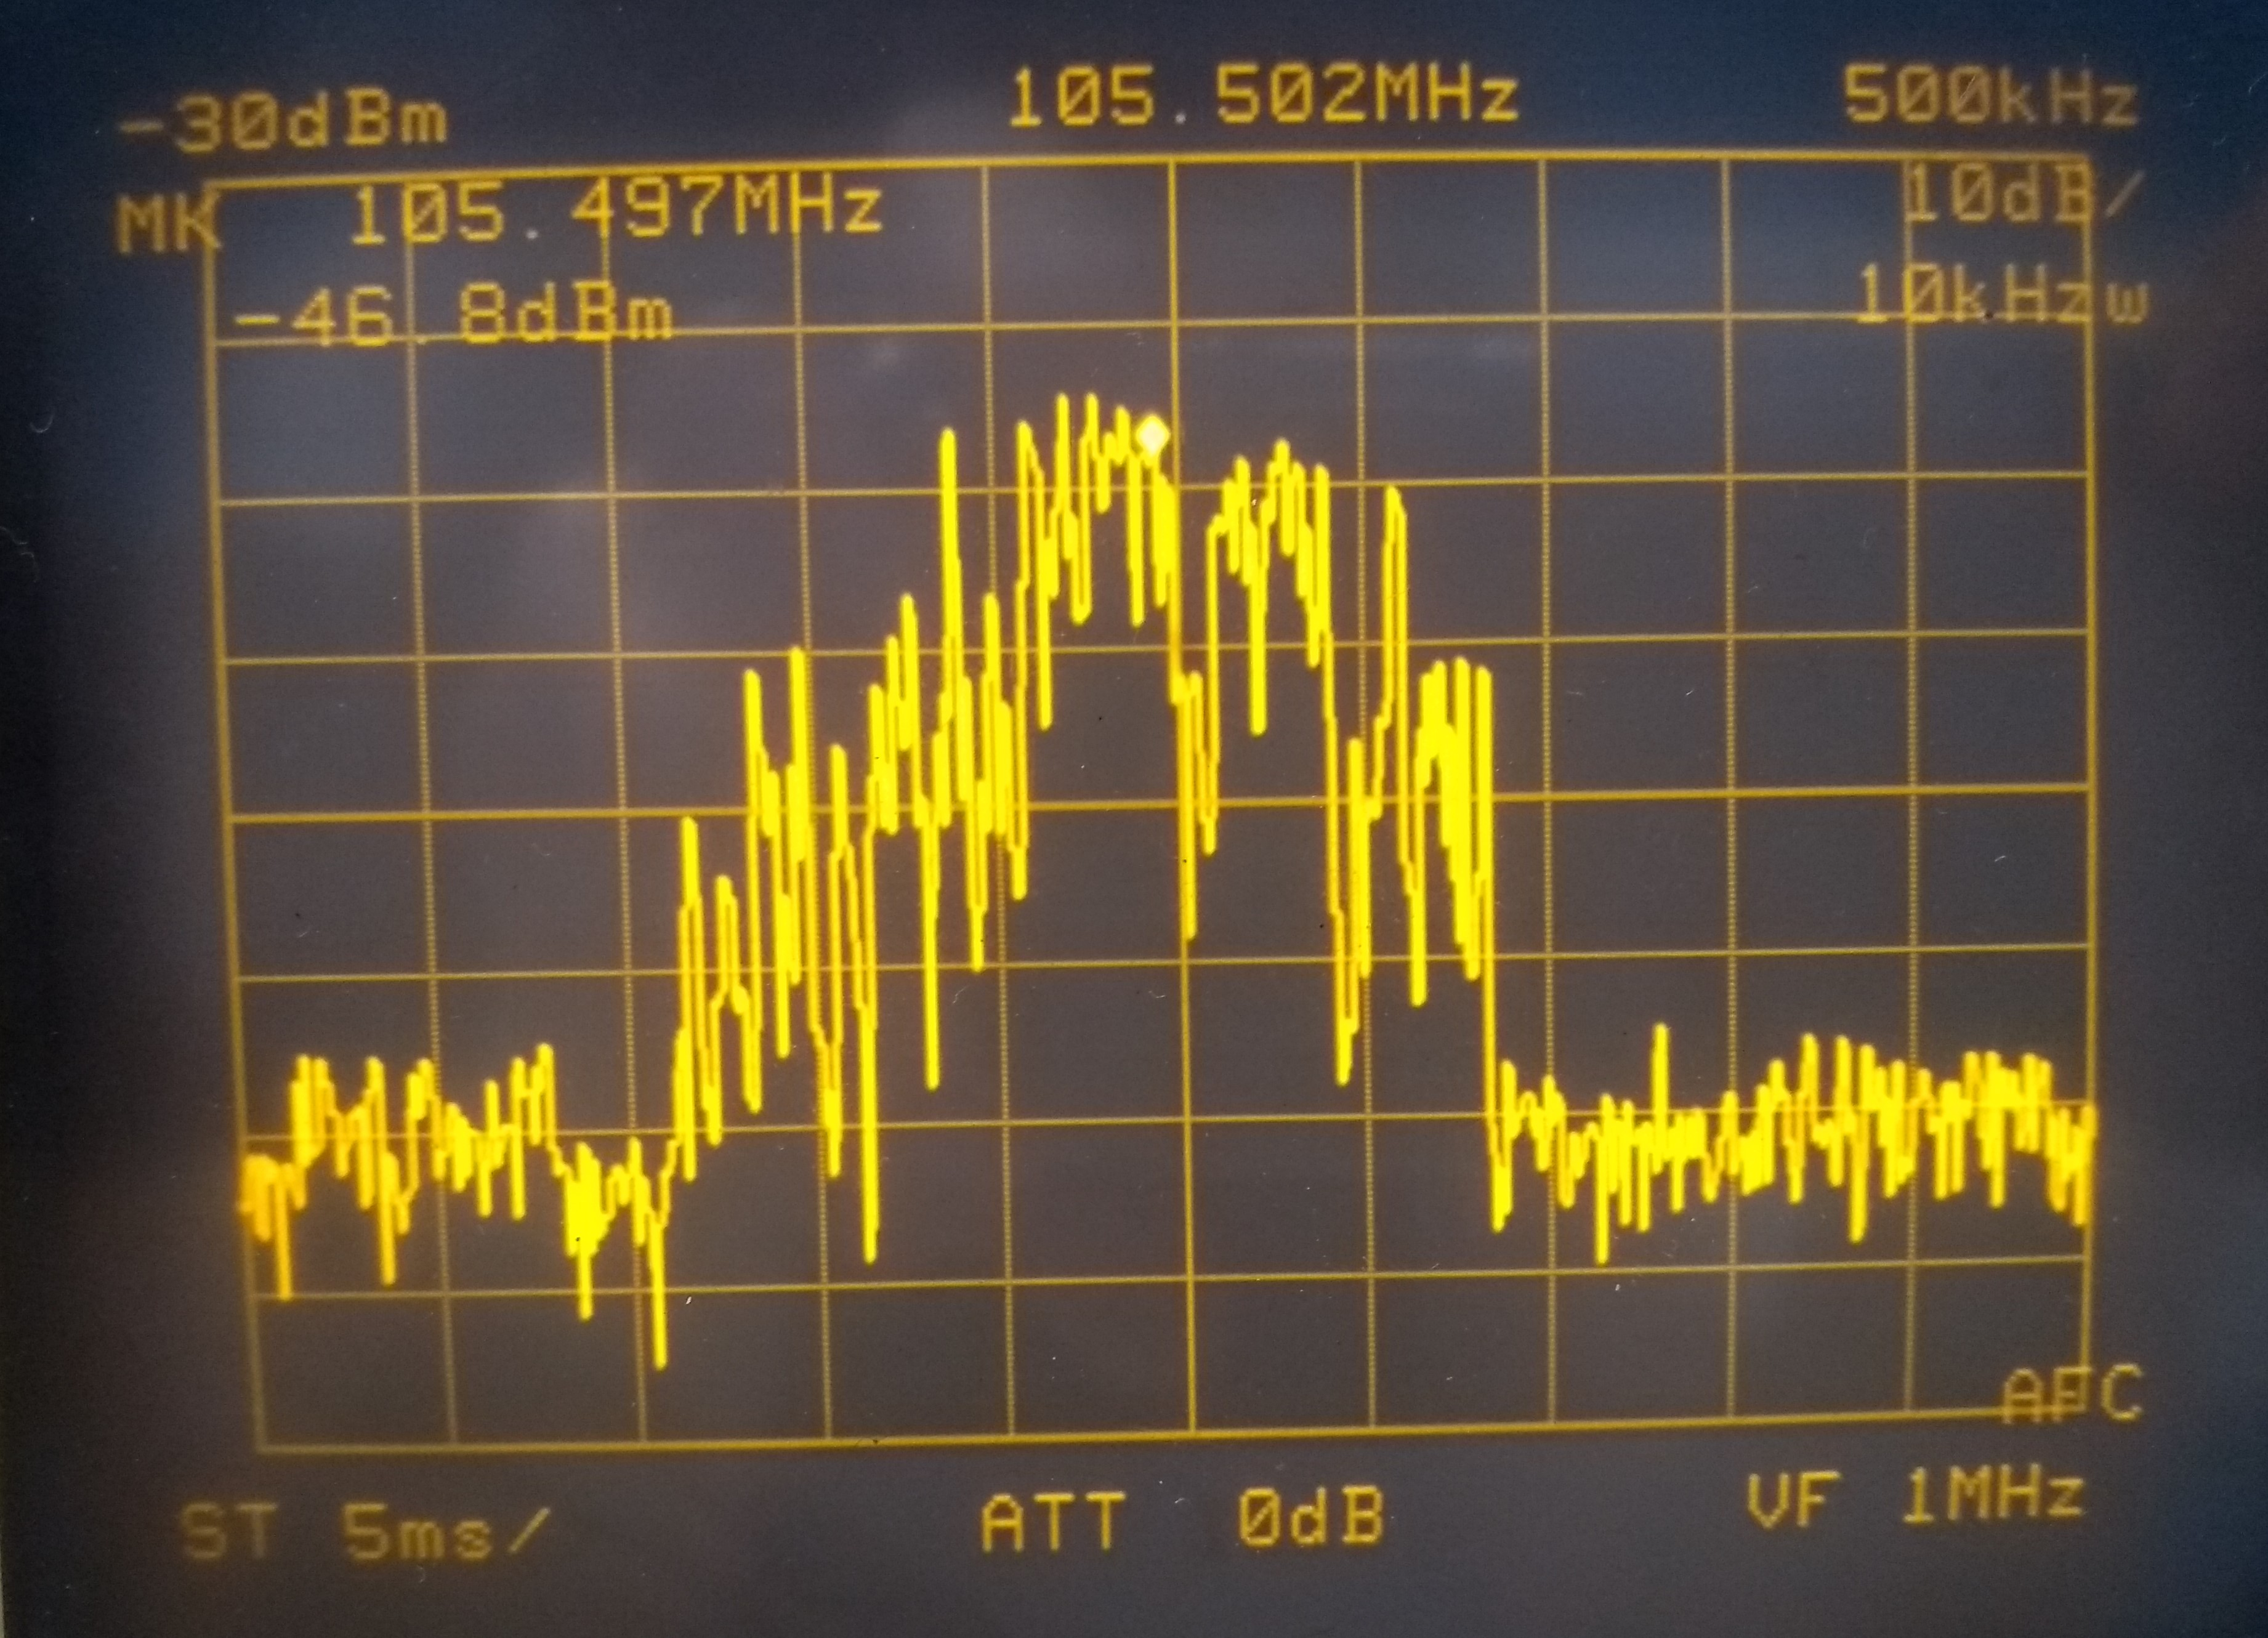
\includegraphics[scale=0.07]{imagenes/sintonizacion_fm.jpg}}
	\caption{Sintonizaci\'on a la emisora "Los 40 principales", el cual tiene asignado el canal 288 a 105.5MHz}
\end{figure}



\end{document}
